\documentclass[12pt,a4paper,brazil,abntex2]{article}
\usepackage[utf8]{inputenc}
\usepackage[portuguese]{babel}
\usepackage[T1]{fontenc}
\usepackage{amsmath}
\usepackage{amsfonts}
\usepackage{amssymb}
\usepackage{makeidx}
\usepackage{graphicx}
\usepackage{indentfirst}		% Indenta o primeiro parágrafo de cada seção.
\usepackage{microtype} 			% para melhorias de justificação
\usepackage[left=3cm,right=2cm,top=3cm,bottom=2cm]{geometry}
\usepackage{url}

\usepackage{setspace}
\usepackage{cite}
\usepackage{float}
\usepackage{breakurl}
\usepackage{verbatim}
\usepackage{listings}
\usepackage{xcolor}

\usepackage[hang, flushmargin]{footmisc}
\usepackage[hidelinks, breaklinks=true]{hyperref}
\usepackage{footnotebackref}
\usepackage{nicefrac}
\usepackage{multirow}
\usepackage{rotating}

\definecolor{mGreen}{rgb}{0,0.6,0}
\definecolor{mGray}{rgb}{0.5,0.5,0.5}
\definecolor{mPurple}{rgb}{0.58,0,0.82}
\definecolor{backgroundColour}{rgb}{0.95,0.95,0.92}

\lstdefinestyle{base}{
  language=bash,
  emptylines=1,
  breaklines=true,
  escapechar=~,
  tabsize=2,
  basicstyle=\ttfamily\color{black},
  moredelim=**[is][\color{red}]{@}{@},
  moredelim=**[is][\color{black}]{!!}{!!}
}

\lstdefinestyle{C}{
    backgroundcolor=\color{backgroundColour},   
    commentstyle=\color{mGreen},
    keywordstyle=\color{magenta},
    numberstyle=\tiny\color{mGray},
    stringstyle=\color{mPurple},
    basicstyle=\footnotesize,
    breakatwhitespace=false,         
    breaklines=true,                 
    captionpos=b,                    
    keepspaces=true,                 
    numbers=left,                    
    numbersep=5pt,                  
    showspaces=false,                
    showstringspaces=false,
    showtabs=false,                  
    tabsize=2,
    escapechar=!,
    language=C
}

\lstset{
language=C,   % R code
literate=
	{á}{{\'a}}1
	{à}{{\`a}}1
	{ã}{{\~a}}1
	{é}{{\'e}}1
	{ê}{{\^e}}1
	{í}{{\'i}}1
	{ó}{{\'o}}1
	{õ}{{\~o}}1
	{ú}{{\'u}}1
	{ç}{{\c{c}}}1
}

\begin{document}
\singlespacing
\begin{titlepage}
\begin{center}
\begin{figure}[!htb]
\center
%\includegraphics[scale=0.25]{/home/sadi/Downloads/Curso/Brasao/Sigla.pdf} 
\end{figure}
{\bf  UNIVERSIDADE FEDERAL DE SANTA CATARINA}\\[0.2cm]
{\bf CENTRO TECNOLÓGICO}\\[0.2cm]
{\bf  DEPARTAMENTO DE INFORMÁTICA E ESTATÍSTICA}\\[5.5cm]
{\bf \large PROCESSAMENTO DISTRIBUÍDO USANDO MPI}\\[3.6 cm]
{Sadi Júnior Domingos Jacinto}\\[1cm]
{Professor orientador: Odorico Machado Mendizabal}\\[4.9 cm]
{Florianópolis}\\[0.2cm]
{2019}
\newpage
\thispagestyle{empty}
{Sadi Júnior Domingos Jacinto}\\[9cm]
{\bf \large PROCESSAMENTO DISTRIBUÍDO USANDO MPI}\\[0.5cm]
    \begin{flushright}
    \begin{list}{}{
      \setlength{\leftmargin}{7.2cm}
      \setlength{\rightmargin}{0cm}
      \setlength{\labelwidth}{0pt}
      \setlength{\labelsep}{\leftmargin}}
      \item Análise do uso de processamento distribuído utilizando MPI, requerido pelo professor da disciplina Programação Paralela e Distribuída, Odorico Machado Mendizabal, necessário para obtenção de nota.\\[0.2 cm] 
      \setlength{\labelsep}{\leftmargin}
      \item Professor orientador: Odorico Machado Mendizabal\
      \\[9cm]
     \end{list}
	 \end{flushright}
{Florianópolis}\\[0.2cm]
{2019}
\end{center}
\end{titlepage} %término da capa
\newpage
\thispagestyle{empty}
\tableofcontents
\section{\normalsize RESUMO}
	Muitos problemas interessantes de otimização não podem ser resolvidos de forma exata, utilizando a computação convencional (sequencial) dentro de um tempo razoável, inviabilizando sua utilização em muitas aplicações reais. 
	
	Embora os computadores estejam cada vez mais velozes, existem limites físicos e a velocidade dos circuitos não pode continuar melhorando indefinidamente. Por outro lado nos últimos anos tem-se observado uma crescente aceitação e uso de implementações paralelas nas aplicações de alto desempenho como também nas de propósito geral, motivados pelo surgimento de novas arquiteturas que integram dezenas de processadores rápidos e de baixo custo. 
	
	Dito isso, o presente relatório tem por objetivo analisar o desempenho de uma aplicação de ordenação de vetores de inteiros em sua implementação paralela, utilizando o MPI para troca de mensagens entre diferentes processos.
\section{\normalsize DEFINIÇÃO DO ESTUDO}
	O presente relatório buscará analisar o desempenho de uma aplicação responsável por ordenar um vetor de inteiros em sua implementação paralela em comparação com sua implementação sequencial.
	
	Para isso, os seguintes critérios foram seguidos:
	\begin{itemize}
		\item A aplicação foi inteiramente escrita na linguagem C.
		\item Foi utilizada a biblioteca OpenMPI para realizar a comunicação entre os diferentes processos.
		\item O algoritmo de ordenação usado foi o \textit{bucket sort}, para a classificação dos dados, e a função \textit{qsort()} para a ordenação dos mesmos.
		\item Tanto a versão paralela quanto a versão sequencial ordenam o mesmo conjunto de dados (copiados para ambas as versões) e utilizam o mesmo número de \textit{buckets}, com o objetivo de os resultados não serem prejudicados por diferenças nas implementações\footnote{afora o paralelismo, é claro.}. 
		\item Foram escritos duas aplicação para realizar essa análise, uma delas dando prioridade para o processamento dos dados e outra priorizando a otimização de memória.
	\end{itemize}
	
	Tais critérios serão melhor explicados ao longo do relatório.
\section{\normalsize MPI (\textit{MESSAGE PASSING INTERFACE})}
	O  MPI é um padrão de interface para a troca de mensagens em máquinas paralelas com memória distribuída. Apesar de alguns pensarem dessa forma, o MPI não é um compilador ou um produto específico.
	
	No padrão MPI, uma aplicação é constituída por um ou mais processos que se comunicam, acionando-se funções para o envio e recebimento de mensagens entre os processos. Inicialmente, na maioria das implementações, um conjunto fixo de processos é criado. Porém, esses processos podem executar diferentes programas. Por isso, o padrão MPI é algumas vezes referido como MPMD (\textit{Multiple Program Multiple Data}).

Elementos importantes em implementações paralelas são a comunicação de dados entre processos paralelos e o balanceamento da carga. É importante frisar que o número de processos no MPI normalmente é fixo. Dito isso, tais processos podem usar mecanismos de comunicação ponto a ponto (operações para enviar mensagens de um determinado processo a outro), ou coletivas, na qual um grupo de processos pode invocar operações coletivas de comunicação para executar operações globais. 

Sobre o MPI, o mesmo é capaz de suportar comunicação assíncrona e programação modular, através de mecanismos de comunicadores que permitem ao usuário MPI definir módulos que encapsulem estruturas de comunicação interna.

Finalmente, os algoritmos que criam um processo para cada processador podem ser implementados, diretamente, utilizando-se comunicação ponto a ponto ou coletivas, sendo que os algoritmos que implementam a criação de tarefas dinâmicas ou que garantem a execução concorrente de muitas tarefas, num único processador, precisam de um refinamento nas implementações com o MPI.
\section{\normalsize \textit{BUCKET SORT}}\label{bucket}
	O \textit{Bucket sort} é uma técnica de classificação que classifica os elementos primeiro os dividindo em vários grupos chamados baldes\footnote{ou \textit{buckets} em inglês, daí o nome.}. Os elementos dentro de cada grupo são classificados usando qualquer um dos algoritmos de classificação adequados ou chamando recursivamente o mesmo algoritmo.

Vários \textit{buckets}\footnote{deste ponto em diante, o termo \textit{bucket} será utilizado ao invés do termo balde.} são criados. Cada \textit{bucket} é preenchido com um intervalo específico de elementos, que então são  classificados usando qualquer outro algoritmo. Por fim, os elementos de cada \textit{bucket} são reunidos para obter a matriz ou o vetor original classificado.

O processo de classificação pode ser entendido como uma abordagem de coleta dispersa. Os elementos são primeiro dispersos em \textit{buckets} e, em seguida, os elementos dos \textit{buckets} são classificados. Finalmente, os elementos são reunidos em ordem.

Esse algoritmo é especialmente útil, e fácil de implementar, em aplicações paralelas, onde cada \textit{bucket} pode ser enviado para um processo, onde o mesmo ordenará o \textit{bucket} e o reenviará, já ordenado, para o processo de origem, o que poderá, dependendo de uma série de fatores, acarretar em um aumento de desempenho com relação à sua implementação sequencial.

	\subsection{\normalsize CLASSIFICAÇÃO DOS \textit{BUCKETS}}\label{classification}
		Os elementos podem ser classificados através de uma função matemática que, dados os valores máximos e mínimos dos elementos, além do número de \textit{buckets} disponível, determina para qual \textit{bucket} tal elemento será enviado.
		
		Essa classificação, apesar de adicionar mais processamento ao algoritmo, garante que, após a ordenação de todos os \textit{buckets}, ao agrega-los, do \textit{bucket} de menor índice (0) até o maior (\textit{n}), o vetor já se encontre ordenado, uma vez que cada \textit{bucket} conterá  um intervalo de elementos que sempre será superior ao \textit{bucket} anterior\footnote{com exceção do \textit{bucket} 0} e inferior ao \textit{bucket} seguinte\footnote{com exceção do último \textit{bucket}}.
		
		As imagens a seguir ilustram melhor isso:
		\begin{figure}[H]
			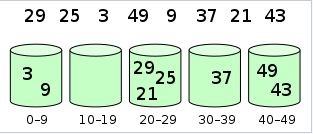
\includegraphics[scale=1]{pictures/01}
		\end{figure}
		
		\begin{figure}[H]
			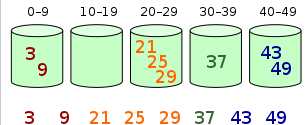
\includegraphics[scale=1]{pictures/02}
		\end{figure}
		
		A função matemática que é usada para calcular em qual \textit{bucket} o elemento deve ser inserido é:
		$$\cfrac{elem - min}{\frac{max - min + 1}{buckets}}$$
		
		Onde:
		\begin{itemize}
			\item elem: é o elemento que se deseja inserir em algum \textit{bucket};
			\item min: menor elemento presente no vetor ou matriz;
			\item max: maior elemento presente no vetor ou matriz e
			\item buckets: número total de \textit{buckets} existentes.
		\end{itemize}
		
	\subsection{\normalsize COMPLEXIDADE}\label{complex}
		\begin{itemize}
			\item \textbf{Pior Complexidade ($\theta(n^{2})$)}:\\
				Quando a distribuição dos elementos não for uniforme, os mesmos provavelmente serão colocados no mesmo \textit{bucket}. Isso pode resultar em alguns \textit{buckets} com mais número de elementos do que outros, o que irá atrasar a execução consideravelmente.
				
				Nesse cenário, a complexidade passa a depender do algoritmo de ordenação usado para ordenar os elementos do \textit{bucket}.
				
				A complexidade se torna ainda pior quando os elementos estão na ordem inversa.
			
			\item \textbf{Melhor Complexidade ($\theta(n + k)$)}:\\
				Ocorre quando os elementos são distribuídos uniformemente nos \textit{buckets}, com um número quase igual de elementos em cada \textit{bucket}.
				
				A complexidade se torna ainda melhor se os elementos dentro dos \textit{buckets} já estiverem classificados.

				Se o algoritmo de ordenação utilizado for de tempo linear, a complexidade geral, na melhor das hipóteses, será linear, isto é, $\theta(n + k)$, onde $\theta(n)$ representa a complexidade para inserir os elementos nos \textit{buckets} e $\theta(k)$ representa a complexidade para ordenar os elementos do \textit{bucket}\footnote{considerando que os algoritmos usados são de complexidade de tempo linear}.
				
			\item \textbf{Caso Médio ($\theta(n)$)}:\\
				Isso ocorre quando os elementos são distribuídos aleatoriamente na matriz. Mesmo que os elementos não sejam distribuídos uniformemente, a classificação do \textit{bucket} é executada em tempo linear.
		\end{itemize}
\section{\normalsize qsort()}
	Trata-se de uma função disponibilizada pela biblioteca \textit{stdlib.h}
\section{\normalsize SOBRE A IMPLEMENTAÇÃO}
\section{\normalsize RESULTADOS}
	Após todo esse detalhamento, ambas as implementações foram submetidas à uma bateria de testes. O ambiente de testes possuí as seguintes configurações:
	
\begin{lstlisting}[frame=single,style=base]
@OS@
Linux s-pc 4.19.85-1-MANJARO #1 SMP PREEMPT Thu Nov 21 10:38:39 UTC 2019 x86_64 GNU/Linux

@CPU@
Architecture:                    x86_64
CPU op-mode(s):                  32-bit, 64-bit
Byte Order:                      Little Endian
Address sizes:                   39 bits physical, 48 bits virtual
CPU(s):                          8
On-line CPU(s) list:             0-7
Thread(s) per core:              1
Core(s) per socket:              8
Socket(s):                       1
NUMA node(s):                    1
Vendor ID:                       GenuineIntel
CPU family:                      6
Model:                           158
Model name:                      Intel(R) Core(TM) i7-9700K CPU !!~@~!! 3.60GHz
Stepping:                        12
CPU MHz:                         800.041
CPU max MHz:                     4900,0000
CPU min MHz:                     800,0000
BogoMIPS:                        7202.00
Virtualization:                  VT-x
L1d cache:                       256 KiB
L1i cache:                       256 KiB
L2 cache:                        2 MiB
L3 cache:                        12 MiB
NUMA node0 CPU(s):               0-7

@RAM@
			total			used		free		shared	buff/cache	available
Mem:	32880560	4269840	14884996	220864	13725724	27972388
Swap:	17408220	0				17408220
\end{lstlisting}

	Além disso, o seguinte \textit{script} foi utilizado para automatizar os testes:

\begin{lstlisting}[language=bash,tabsize=2]
#!/bin/bash

if [ ! -f "memory" ]; then
	mpicc -o memory mpi_memory_priority.c
fi

if [ ! -d "process" ]; then
	mpicc -o process mpi_process_priority.c
fi

for h in {1..10}; do
	for i in "memory" "process"; do
		for j in {1..8}; do
			for k in 10 100 1000 10000 100000 1000000 10000000 100000000
			 1000000000 2147483647; do
				mpirun --use-hwthread-cpus -np "$j" "$i" "$k" &>> 
				"$i"_results.txt 
			done
		done
	done
done
\end{lstlisting}

	É importante ressaltar que esse \textit{script}, além de testar a execução das aplicações com diferentes quantidades de processos e tamanhos de vetor, também executa a mesma ação várias vezes, de forma a aumentar a precisão dos resultados. Outro detalhe importante é que o valor 2147483647, passado como último parâmetro na lista de tamanhos de vetores, é exatamente o maior valor que o tipo \textit{int} em C consegue armazenar.
	
	Assim, após várias execuções e uma posterior análise dos resultados, as médias encontradas foram as seguintes (em segundos):

%\begin{sidewaystable}
\begin{flushleft}
{\tiny
\begin{tabular}{|p{1.5cm}|p{1.2cm}|p{1.3cm}|p{1.3cm}|p{1.3cm}|p{1.3cm}|p{1.3cm}|p{1.3cm}|p{1.3cm}|p{1.3cm}|}
\hline
Implementação & \multirow{2}{*}{Vetor} & \multicolumn{8}{|c|}{Número de Processos}\\\cline{3-10}\cline{1-1}
\multirow{9}{*}{\shortstack[l]{Paralela com \\gerência de \\memória}} 
& 								& 1 									& 	2 									& 3 									& 4 									& 5 									& 6 									& 7 							& 8					\\\cline{2-10}
& 10 						& 	.0000027 		& .0000212 			& .0000415 			&  .0000903 		&  .0000934 		&  .0001560			&  .0001146 &  .0019275					\\\cline{2-10}
&100 						&  1.0563653 		& .1112110 			& .0826674 			& .0507492 			& .0436394 			& .0395596 			& .0255500 & .0174826						\\\cline{2-10}
&1000 					& 	.8000998 		& .3594714 			& .2369371 			& .1673131 			& .1553424 			& .1354610 			& .0777393 & .0578452					\\\cline{2-10}
&10000 				& 	.9741429 			& 1.2666282 		& 1.2195104 		& .9837416 			& .9791490 			& .8325129 			& .5492519 & .2605338					\\\cline{2-10}
&100000 				& 	.9860416 			& 1.5651301 		& 2.0407331 		& 2.2999293 		& 2.1712966 		& 2.0481064 		& 1.0838959 & .9847480					\\\cline{2-10}
&1000000			& 	.9607970 			& 1.5388010 		& 1.9747255 		& 1.9323342 		& 2.4203360 		& 2.6410168 		& 2.7246242 & 2.2595285					\\\cline{2-10}
&10000000 		& 	2.7605220 		& 2.7235129 		& 3.0418588 		& 3.4210596 		& 3.7121727 			& 4.0453188 		& 4.3461586 & 4.4894687					\\\cline{2-10}
&100000000 		& 	20.0093707 	& 11.9920976 		& 9.7144958 		& 8.8905494 		& 8.5092091 		& 8.4090180 		& 8.3337478 & 8.3078605					\\\cline{2-10}
&1000000000	& 	201.1842203 	& 108.8012184 	& 77.8979812 		& 64.2787633 	& 55.5181042 		& 50.6841951		& 47.0156535 & 44.7843406					\\\cline{2-10}
&2147483647		& 	446.4906463 	& 446.1086100 	& 273.6945712 	& 257.1397809 	& 230.8994899 	& 220.2747467	& 236.7602789 & 244.1795316					\\\hline

\rule{0pt}{4ex}\multirow{9}{*}{\shortstack[l]{Paralela sem \\gerência de \\memória}} 
%&							& 1 							& 	2 									& 3 									& 4 									& 5 									& 6 									& 7 										& 8
& 10 						& 	.0000030 		& .0000271000 			& .0000476000 		& .0000949000 		& .0000673000 		& .0000656000 		& .0002626000 				& .0012136000				\\\cline{2-10}
&100 						&  .9837493 		& .0862721000 			& .0716700000 			& .0462184000 			& .0538141000 			& .0369232000 			& .0245561000 				& .0157813000				\\\cline{2-10}
&1000 					& 	.8231967 			& .3134539000 			& .3955453000 			& .2186298000 			& .1562831000 			& .1135984000 			& .0688420000 				& .0642171000				\\\cline{2-10}
&10000 				& 	.9168636 			& 1.2575031000 		& 1.4855136000 		& 1.1014654000 		& .9419980000 			& .9094361000 			& .4372316000 				& .3478161000				\\\cline{2-10}
&100000 				& 	.9768038 			& 1.6550726000 		& 2.1703707000 		& 2.2497163000 		& 2.3273306000 		& 2.3491862000 		& 1.5417702000 			& 1.2046256000					\\\cline{2-10}
&1000000			& 	.9694479 			& 1.4762001000 		& 2.0421743000 		& 2.4354964000 		& 2.4395516000 		& 2.8496056000 		& 2.9251988000 			& 2.3478941000				\\\cline{2-10}
&10000000 		& 	2.7014685		 & 2.7044231000 		& 3.1015553000 		& 3.5178755000 		& 3.9416155000 		& 4.3603101000 		& 4.7265146000 			& 5.0408849000				\\\cline{2-10}
&100000000 		& 	19.5167693 		& 11.5480279000 		& 9.3549584000 		& 8.6173853000 		& 8.3163671000 		& 8.3046885000 		& 8.3152313000 			& 8.3754224000				\\\cline{2-10}
&1000000000	& 	195.8188751 	& 103.9194018000 	& 73.4289533000 	& 59.8611877000 		& 51.2025075000 		& 46.3851032000 		& 42.7621825000 			& 40.4988312000				\\\cline{2-10}
&2147483647		& 	434.6594085	 & 410.4079653000	 & 265.4520660000 & 240.0495133000 	& 218.0640578000 	& 210.2243664000 	& 223.0438916000 		& 249.1748597000				\\\hline

\rule{0pt}{4ex}\multirow{9}{*}{\shortstack[l]{Sequencial com \\gerência de \\memória}} 
%& 						& 1 									& 	2 									& 3 									& 4 									& 5 									& 6 									& 7 									& 8
& 10 						& 	.0000025000 		& .0000022000 		& .0000031000 			& .0000038000 		& .0000033000 		& .0000048000 		& .0000028000 		& .0000047000				\\\cline{2-10}
&100 						&  .0000088000 		& .0000091000 			& .0000083000 		& .0000090000 		& .0000074000 		& .0000081000 			& .0000080000 		& .0000087000				\\\cline{2-10}
&1000 					& 	.0001089000 			& .0001284000 			& .0001330000 			& .0000930000 		& .0001158000 			& .0001213000 			& .0001040000 		& .0001059000				\\\cline{2-10}
&10000 				& 	.0013649000 			& .0023878000 			& .0015814000 			& .0015632000 			& .0017591000 			& .0022764000 			& .0014967000 			& .0012290000					\\\cline{2-10}
&100000 				& 	.0147589000 			& .0158598000 			& .0167120000 			& .0196422000 			& .0169868000 			& .0163800000 			& .0148048000 			& .0133163000					\\\cline{2-10}
&1000000			& 	.1540481000 			& .1494087000 			& .1466629000 			& .1458039000 			& .1432673000 			& .1422641000 			& .1412189000 			& .1394688000					\\\cline{2-10}
&10000000 		& 	1.7733550000 		& 1.7256406000 		& 1.6878593000 		& 1.6779745000 		& 1.6618811000 			& 1.6680603000 		& 1.6461618000 		& 1.6309406000				\\\cline{2-10}
&100000000 		& 	19.0142680000 		& 18.6113519000 		& 18.2048137000		& 18.1662202000 		& 18.0164274000 		& 18.1155132000 		& 17.9767386000 		& 17.7508518000				\\\cline{2-10}
&1000000000	& 	200.1272696000 	& 196.2480242000 	& 191.0897795000 	& 191.9411290000 	& 189.1976788000 	& 190.5518217000 	& 189.6506084000 	& 188.0026819000				\\\cline{2-10}
&2147483647		& 	445.1986421000 	& 433.9378432000 	& 425.9063507000 	& 428.7750298000 	& 425.2087999000 	& 426.9832087000 	& 424.7350147000 	& 421.8411051000				\\\hline

\rule{0pt}{4ex}\multirow{9}{*}{\shortstack[l]{Sequencial sem \\gerência de \\memória}} 
%& 						& 1 									& 	2 									& 3 									& 4 									& 5 									& 6 									& 7 									& 8
& 10 						& 	.0000027000 		& .0000018000 			& .0000028000 		& .0000032000 		& .0000034000 		& .0000021000 			& .0000021000 			& .0000025000				\\\cline{2-10}
&100 						&  .0000081000 		& .0000075000 		& .0000089000 		& .0000076000 		& .0000075000 		& .0000100000 		& .0000062000 		& .0000072000				\\\cline{2-10}
&1000 					& 	.0000968000 		& .0000953000 		& .0001162000 			& .0000849000 		& .0001482000 			& .0001188000 			& .0001094000 			& .0001103000				\\\cline{2-10}
&10000 				& 	.0014130000 			& .0013441000 			& .0016208000 			& .0020205000 			& .0017560000 			& .0016613000 			& .0015043000 			& .0012711000				\\\cline{2-10}
&100000 				& 	.0143784000 			& .0160259000 			& .0159414000 			& .0156171000 			& .0192616000 			& .0175861000 			& .0147695000 			& .0130214000				\\\cline{2-10}
&1000000			& 	.1498177000 			& .1446836000 			& .1419181000 			& .1410430000 			& .1388499000 			& .1378981000 			& .1368962000 			& .1350305000				\\\cline{2-10}
&10000000 		& 	1.7231449000 		& 1.6751685000 		& 1.6402247000 		& 1.6320957000 		& 1.6153452000 		& 1.6234146000 		& 1.6010744000 		& 1.5869500000					\\\cline{2-10}
&100000000 		& 	18.4980438000 	& 18.1018721000 		& 17.7414867000 		& 17.7155829000 		& 17.5760846000 		& 17.6640543000 	& 17.5282711000 		& 17.3022210000					\\\cline{2-10}
&1000000000	& 	195.0625062000 	& 191.0199901000 	& 186.5348480000 	& 187.4723130000 	& 184.7847845000 	& 186.0704603000 	& 185.2330530000 	& 183.4975351000				\\\cline{2-10}
&2147483647		& 	433.7706016000 	& 423.0627653000 	& 416.3450064000 	& 417.9715770000 	& 415.6978661000 	& 417.8453379000 	& 415.2326078000 	& 413.5186273000					\\\hline

\rule{0pt}{4ex}\multirow{9}{*}{\shortstack[l]{\textit{Speedup} com\\gerência de \\memória}} 
%& 						& 1 								& 	2 								& 3 								& 4 								& 5 								& 6 								& 7 								& 8
& 10 						& 	1.0563538000 	& .1111796000 		& .0826103000 		& .0506783000 		& .0435639000 		& .0394951000 		& .0253658000 		& .0164507000					\\\cline{2-10}
&100 						& .7999870000 		& .3593677000 		& .2368266000 		& .1672092000 		& .1552258000 		& .1352418000 		& .0770833000 		& .0530964000				\\\cline{2-10}
&1000 					& 	.9727282000 		& 1.2650407000 	& 1.2187299000 	& .9830587000 		& .9782104000 		& .8311917000 		& .5452368000 		& .2568344000					\\\cline{2-10}
&10000 				& 	.9666650000 		& 1.5534864000 	& 2.0312218000 	& 2.2890732000 	& 2.1635214000 	& 2.0413535000 	& 1.0781567000 	& .9779498000				\\\cline{2-10}
&100000 				& 	.8028554000 		& 1.4544115000 	& 1.9125609000 	& 1.8814876000 	& 2.3760855000 	& 2.6016920000 	& 2.6889351000 	& 2.2257165000				\\\cline{2-10}
&1000000			& 	.9753687000 		& 1.7706385000 	& 2.3604424000 	& 2.8685099000 	& 3.2385253000 	& 3.6183081000 	& 3.9578905000 	& 4.1291774000				\\\cline{2-10}
&10000000 		& 	.9938122000 		& 1.8109971000 	& 2.4769933000 	& 3.0368172000 	& 3.5087097000 	& 3.9063703000 	& 4.2397618000 	& 4.5267375000				\\\cline{2-10}
&100000000 		& 	.9999014000 		& 1.8280400000 	& 2.5154829000 	& 3.1033716000 	& 3.6029296000 	& 4.0233062000 	& 4.3910152000 	& 4.6945991000				\\\cline{2-10}
&1000000000	& 	.9997197000 		& 1.8345691000 	& 2.5349737000 	& 3.1375610000 	& 3.6443662000 	& 4.0837618000 	& 4.4493578000 	& 4.6896176000			\\\cline{2-10}
&2147483647		& 	.9993203000 		& .9981308000 		& 1.5738492000 	& 1.6963718000 	& 1.8716650000 	& 1.9762450000 	& 1.8352416000 	& 1.7833164000					\\\hline


\rule{0pt}{4ex}\multirow{9}{*}{\shortstack[l]{\textit{Speedup} sem\\gerência de \\memória}} 
%& 						& 1 								& 	2 								& 3 								& 4 								& 5 								& 6 								& 7 								& 8
& 10 						& 	.9837395000 		& .0862420000 		& .0716416000 		& .0461688000 		& .0537533000 		& .0366467000 		& .0244397000 		& .0154681000					\\\cline{2-10}
&100 						&  .8230913000 		& .3133785000 		& .3954601000 		& .2185500000 		& .1561254000 		& .1134673000 		& .0674693000 		& .0618467000				\\\cline{2-10}
&1000 					& 	.9153362000 		& 1.2566842000 	& 1.4847572000 	& 1.1004304000 	& .9411215000 		& .9085120000 		& .4342385000 		& .3456651000				\\\cline{2-10}
&10000 				& 	.9577685000 		& 1.6425605000 	& 2.1615725000 	& 2.2428374000 	& 2.3191601000 	& 2.3425181000 	& 1.5358784000 	& 1.1978571000				\\\cline{2-10}
&100000 				& 	.8162057000 		& 1.3958345000 	& 1.9846553000 	& 2.3886439000 	& 2.4000235000 	& 2.8149528000 	& 2.8939701000 	& 2.3193233000					\\\cline{2-10}
&1000000			& 	.9776762000 		& 1.8005381000 	& 2.4680613000 	& 3.0119530000 	& 3.5139316000 	& 3.9801200000 	& 4.3849021000 	& 4.7272835000					\\\cline{2-10}
&10000000 		& 	.9996348000 		& 1.8533001000 	& 2.5891922000 	& 3.2259835000 	& 3.7769679000 	& 4.2700123000 	& 4.6868246000 	& 5.0604125000				\\\cline{2-10}
&100000000 		& 		.9990141000 	& 1.8671916000 	& 2.6222517000 	& 3.2859000000 	& 3.8719115000 	& 4.3780682000 	& 4.8308537000 	& 5.2193626000					\\\cline{2-10}
&1000000000	& 	1.0012484000 	& 1.8717926000 	& 2.6344281000 	& 3.3136805000 	& 3.9041432000 	& 4.4295172000 	& 4.8834218000 	& 5.2012982000				\\\cline{2-10}
&2147483647		& 	1.0002595000 	& 1.0371885000	 	& 1.5904147000 	& 1.7749154000 	& 1.9415884000 	& 2.0323065000 	& 1.9134115000 		& 1.7141855000				\\\hline
\end{tabular}
}
\end{flushleft}
%\end{sidewaystable}

\subsection{\normalsize ALGUMAS CONSIDERAÇÕES}
	\begin{itemize}
		\item A inicialização do MPI é realizada antes de se iniciar a análise do tempo de processamento.
		
		\item A alocação de memória para o vetor original assim como a inserção de elementos aleatórios no mesmo, tanto na versão paralela quanto na sequencial, são realizadas antes de se iniciar a análise do tempo de processamento 

		\item Todos os \textit{outputs} da aplicação estão inseridos em partes do código nas quais ou a análise de tempo de processamento já encerrou ou a mesma ainda não foi iniciada, de forma que tais \textit{outputs} em nada interferem no desempenho final da aplicação.

		\item Os \textit{outputs} que mostravam o vetor antes e depois de ser ordenado, tanto na versão paralela quanto na sequencial, apesar de estarem em partes não críticas do código\footnote{vide item superior} foram comentados para evitar poluição visual\footnote{em casos de vetores com tamanho elevado}. Os mesmos podem ser descomentados à vontade.
	\end{itemize}
\include{Conclusões}
\end{document}
